\section{Конструкторская часть}

\subsection{Структура ftrace\_ops и функция коллбека}

Для регистрации функции коллбека необходима структура ftrace\_ops~\cite{ftrace_hook}. Структура приведена в листинге~\ref{lst:ftraceops}.

\begin{lstlisting}[label={lst:ftraceops}, caption={структура ftrace\_ops}]
	struct ftrace_ops ops = {
		.func    = callback_func,
		.flags   = FTRACE_FLAGS
		.private = any_private_data_structure,
	};
\end{lstlisting}

Эта структура используется, чтобы сообщить ftrace, какую функцию следует вызывать в качестве коллбека, а также какие меры защиты будут выполняться коллбеком. Поля flags и private являются необязательными.

Включение отслеживания вызовов:

\begin{lstlisting}
	register_ftrace_function(&ops);
\end{lstlisting}

Отключение отслеживания вызовов:

\begin{lstlisting}
	unregister_ftrace_function(&ops);
\end{lstlisting}

Прототип функции коллбека выглядит следующим образом:

\begin{lstlisting}
	void callback_func(unsigned long ip, unsigned long parent_ip, struct ftrace_ops *op, struct pt_regs *regs);
\end{lstlisting}

\begin{itemize}
	\item ip -- указатель инструкции перехватываемой функции;
	
	\item parent\_ip -- указатель инструкции функции, вызвавшей перехватываемую функцию;
	
	\item op -- указатель на ftrace\_ops;
	
	\item regs -- если в структуре ftrace\_ops установлены флаги\\ FTRACE\_OPS\_FL\_SAVE\_REGS или\\ FTRACE\_OPS\_FL\_SAVE\_REGS\_IF\_SUPPORTED, то это будет указывать на структуру pt\_regs, как если бы точка останова была размещена в начале функции, которую перехватывал ftrace. В противном случае он либо содержит мусор, либо NULL.
\end{itemize}

\subsection{Алгоритм перехвата системного вызова}

На риснуке \ref{fig:ftrace_algo} представлена схема алгоритма перехвата системных вызовов на примере sys\_clone.

\begin{figure}[h]
	\begin{center}
		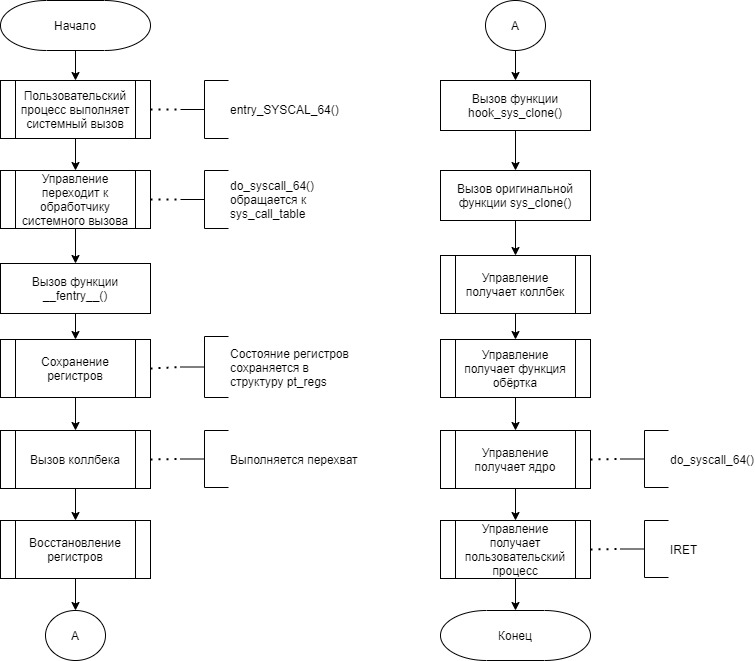
\includegraphics[scale=0.6]{jpg/ftrace_algo.jpg}
	\end{center}
	\caption{Алгоритм перехвата системного вызова}
	\label{fig:ftrace_algo}
\end{figure}

\newpage

\begin{enumerate}
	\item Пользовательский процесс выполняет инструкцию SYSCALL. С помощью этой инструкции выполняется переход в режим ядра и управление передаётся низкоуровневому обработчику системных вызовов\\ entry\_SYSCALL\_64(). Этот обработчик отвечает за все системные вызовы 64-битных программ на 64-битных машинах.
	
	\item Управление переходит к обработчику системного вызова. Ядро передаёт управление функции do\_syscall\_64(). Эта функция обращается к таблице обработчиков системных вызовов sys\_call\_table и с помощью неё вызывает конкретный обработчик системного вызова -- sys\_clone().
	
	\item Вызывается ftrace. В начале каждой функции ядра находится вызов функции \_\_fentry\_\_(), реализованная фреймворком ftrace. Перед этим состояние регистров сохраняется в специальную структуру pt\_regs.
	
	\item ftrace вызывает разработанный коллбек.
	
	\item Коллбек выполняет перехват. Коллбек анализирует значение  parent\_ip и выполняет перехват, обновляя значение регистра rip (указатель на следующую исполняемую инструкцию) в структуре pt\_regs.
	
	\item ftrace восстанавливает значение регистров с помощью структуры pt\_regs. Так как обработчик изменяет значение регистр rip -- это приведёт к передачу управления по новому адресу.
	
	\item Управление получает функция обёртка. Благодаря безусловному переходу, управление получает наша функция hook\_sys\_clone(), а не оригинальная функция sys\_clone(). При этом всё остальное состояние процессора и памяти остаётся без изменений -- функция получает все аргументы оригинального обработчика и при завершении вернёт управление в функцию do\_syscall\_64().
	
	\item Функция обёртка вызывает оригинальную функцию. Функция\\ hook\_sys\_clone() может проанализировать аргументы и контекст системного вызова и запретить или разрешить процессу его выполнение. В случае его запрета, функция просто возвращает код ошибки. Иначе -- вызывает оригинальный обработчик sys\_clone() повторно, с помощью указателя real\_sys\_clone, который был сохранён при настройке перехвата.
	
	\item Управление получает коллбек. Как и при первом вызове sys\_clone(), управление проходит через ftrace и передается в коллбек.
	
	\item Коллбек ничего не делает. В этот раз функция sys\_clone() вызывается разработанной функцией hook\_sys\_clone(), а не ядром из функции\\ do\_syscall\_64(). Коллбек не модифицирует регистры и выполнение функции sys\_clone() продолжается как обычно.
	
	\item Управление передаётся функции обёртке.
	
	\item Управление передаётся ядру. Функция hook\_sys\_clone() завершается и управление переходит к do\_syscall\_64().
	
	\item Управление возвращает в пользовательский процесс. Ядро выполняет инструкцию IRET, устанавливая регистры для нового пользовательского процесса и переводя центральный процессор в режим исполнения пользовательского кода.
\end{enumerate}

\subsection{Алгоритм подсчёта количества системных вызовов}

На риснуке \ref{fig:ftrace_cnt_algo} представлена схема алгоритма подсчёта системных вызовов.

\begin{figure}[h]
	\begin{center}
		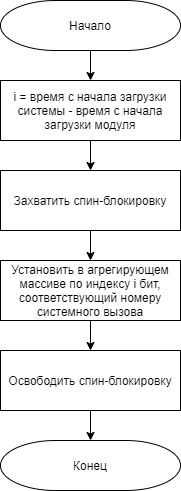
\includegraphics[scale=0.6]{jpg/syscalls_count.jpg}
	\end{center}
	\caption{Алгоритм подсчёта количества системных вызовов}
	\label{fig:ftrace_cnt_algo}
\end{figure}

\newpage

\begin{itemize}
	\item Агрегирующий массив -- это массив на 86400 элементов (что соответствует 24 часам), состоящий из структур, имеющих два поля в виде 64-битных беззнаковых целых чисел. Это позволяет фиксировать до 128 системных вызов в секунду на протяжении 24 часов. Такой массив занимает всего лишь 1350 килобайт оперативной памяти;
	
	\item спин-блокировка необходима с той целью, что несколько системных вызовов могут быть вызваны в один и тот же момент времени -- в таком случае, без блокировки, агрегирующий массив потеряет часть данных.
\end{itemize}

\subsection{Алгоритм получения информации об объеме памяти}

На рисунке \ref{fig:kthread} представлена схема алгоритма работы потока ядра, предназначенного для подсчета объема свободной и занятой оперативной памяти в системе.

\begin{figure}[h!]
	\begin{center}
		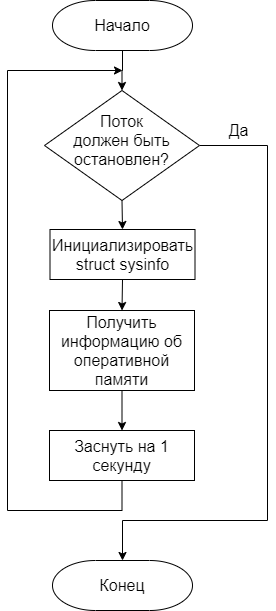
\includegraphics[scale=0.5]{jpg/kthread.png}
	\end{center}
	\captionsetup{justification=centering}
	\caption{Схема алгоритма работы потока}
	\label{fig:kthread}
\end{figure}

\subsection{Точки входа}

Точками входа разрабатываемого загружаемого модуля ядра будут являться функции инициализации и выхода из модуля.

При инициализации модуля будут создаваться необходимые для сохранения результатов директория и файлы в /proc, происходить создание и запуск потока ядра для подсчета объема оперативной памяти и устанавливаться хуки для перехвата системных вызовов.

Функция выхода из модуля в свою очередь будет предназначена для остановки потока, удаления созданных директории и файлов в /proc и удаления установленных хуков.